% Chapter 1: General Project Framework and State of the Art

\chapter{General Project Framework and State of the Art}
\label{ch:chapter1}

\section{Introduction}
This chapter establishes the analytical framework and security context of the project. It examines the data policies of dominant centralized platforms, analyzes the privacy challenges of corporate messaging systems, critiques existing secure protocols, and proposes our client-encrypted, open-source alternative. Additionally, it outlines our Scrum development methodology and secure release plan.


\section{Context and Motivation}
The motivation driving this project is the erosion of personal digital privacy on centralized social platforms. 

\subsection{Critique of Proprietary Data Policies (Discord)}
Proprietary platforms, specifically \textbf{Discord}, enforce data management policies that present significant risks to user privacy:
\begin{itemize}
    \item \tech{Centralized Harvesting}: Chat logs, images, and user files are stored indefinitely in plaintext formats on server databases. 
    \item \tech{Metadata Profiling}: User connection logs, voice channel durations, friendship graphs, and game activities are harvested to build detailed behavioral profiles.
    \item \tech{Commercialization of Conversations}: Corporate terms allow automated data indexing to train language models, optimize ads, and feed corporate brokers, treating private digital spaces as raw commercial assets.
\end{itemize}

\begin{figure}[H]
    \centering
    
\includegraphics[width=0.25\textwidth]{discord.png}
    \caption{Discord Platform.}
    \label{fig:discord}
\end{figure}

\subsection{The Open-Source Necessity}
Addressing this surveillance model requires a transparent, open-source alternative that respects user privacy. Closed-source systems contain unverified security pipelines. Open-source code allows independent auditing of all cryptographic functions, ensuring that no administrative backdoors exist and giving users complete control over their client binaries.

\section{State of the Art and Security Critique}
We analyzed existing enterprise communication tools and secure messaging models to identify architectural weaknesses:

\begin{itemize}
    \item \tech{Discord, Slack, and Microsoft Teams (Centralized SPoF)}: In these architectures, the central servers manage the cryptographic keys and decrypt all payloads for scanning or storage. The server acts as a \textbf{Single Point of Failure (SPoF)}: a single backend database breach, rogue employee, or government subpoena exposes all conversations in plaintext.
\end{itemize}
\section{Market Research Landscape}
The market for real-time communication platforms has shifted dramatically in the last decade, moving from simple text messaging to complex ecosystems supporting voice, video, and real-time collaboration.

According to recent market analysis by Grand View Research, the global unified communications market size was valued at USD 136.11 billion in 2023 and is expected to grow at a compound annual growth rate (CAGR) of 17.4\% from 2024 to 2030 \cite{grandviewucaas}. This growth is primarily driven by the proliferation of remote work and the increasing need for agile team collaboration tools.

Key trends in the current market include:
\begin{itemize}
    \item \textbf{Shift to OTT Applications}: Over-the-top (OTT) messaging applications like WhatsApp, Discord, and Telegram have largely replaced traditional SMS and email for casual and professional communication.
    \item \textbf{Privacy as a Premium Feature}: While early adopters focused on features and speed, a significant segment of the market—estimated at nearly 30\% of enterprise users according to a Gartner survey—now prioritizes data sovereignty and encryption capabilities over convenience.
    \item \textbf{Regulatory Pressure}: Legislation such as GDPR in Europe and CCPA in California is forcing providers to rethink data harvesting strategies, yet many platforms still rely on opaque data mining for revenue.
\end{itemize}

This research indicates a viable gap in the market for a platform that bridges the usability of mainstream apps with the security rigor typically reserved for enterprise-only tools.

\section{Proposed Solution (The Secure Alternative)}
We propose a community communication platform designed to be secure-by-default, balancing robust security with a seamless user experience:
\begin{enumerate}
    \item \tech{Client-Side E2EE Text Chat}: Texts are encrypted on the sender's device before sending over WebSockets. The central database only stores base64-encoded ciphertexts, meaning the server stores \textbf{no plaintext data}.
    \item \tech{WebRTC P2P Voice Channels}: Audio streams flow directly IP-to-IP between peers. The backend acts solely as a neutral signaling relay, and the streams are secured against wiretapping via DTLS and SRTP.
\end{enumerate}

\section{Project Management Methodology (Scrum)}
We chose agile methodologies for the development of our application, as they tend to minimize the software lifecycle by producing successive versions. The application's features are delivered in an iterative process while listening to the client and the tests carried out during the project realization period.

We have adopted the agile SCRUM \cite{scrum_overview} methodology for our project in order to adapt to changes in specifications from the various stakeholders during the development process. SCRUM is based on 3 main foundations:
\begin{itemize}
    \item \textbf{Inspection}: Regular reviews in order to adapt the project if necessary.
    \item \textbf{Adaptation}: The ability to implement new measures when the inspection results are different from what was expected.
    \item \textbf{Transparency}: Every member of the SCRUM team knows the information relating to the product.
\end{itemize}

\begin{figure}[H]
    \centering
    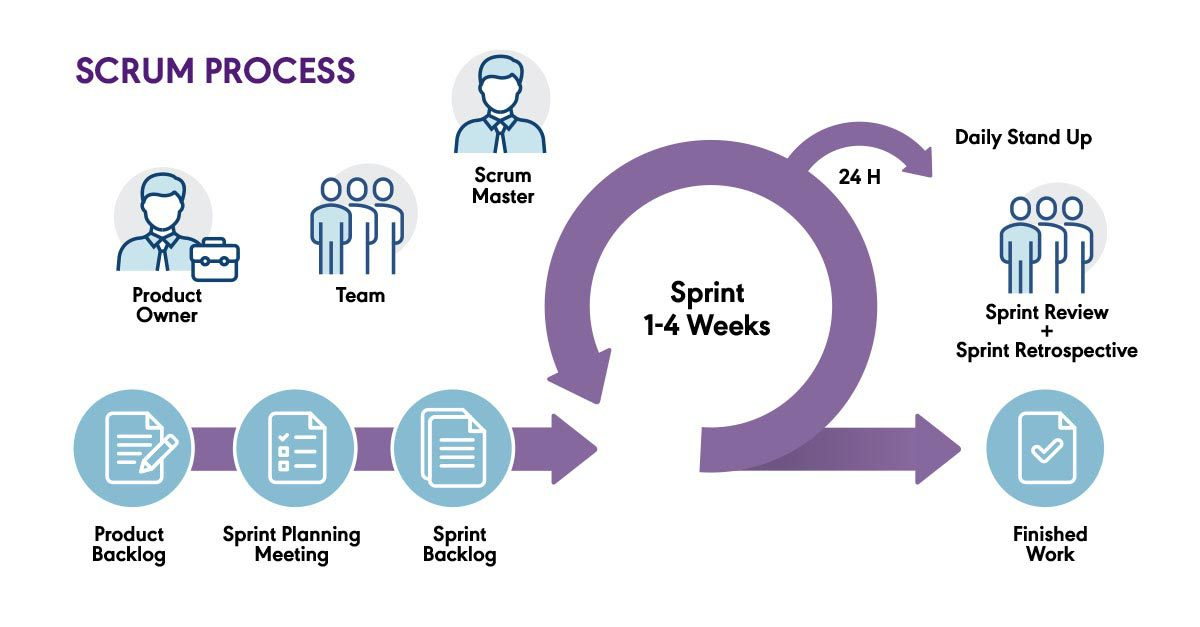
\includegraphics[width=\textwidth]{scrum_process.jpg}
    \caption{Scrum Process Overview \cite{scrum_overview}.}
    \label{fig:scrum_process}
\end{figure}

\begin{table}[H]
    \centering
    \renewcommand{\arraystretch}{1.5}
    \begin{tabular}{|l|p{7cm}|p{4.5cm}|}
        \hline
        \textbf{Role} & \textbf{Description} & \textbf{Actor} \\
        \hline
        Product Owner & Represents the client by defining the requirements and features to be developed & Iteam university \\
        \hline
        SCRUM Master & Guides the SCRUM team and ensures the organization and smooth execution of the SCRUM process & Mme Afef ghabri \\
        \hline
        SCRUM Team & Responsible for the design, development, testing, and implementation of the product & Oussama Dhia Arouay \newline Rayen Barkallah \newline Adem Rokh \newline Mohamed Amine Jebali \\
        \hline
    \end{tabular}
    \caption{Scrum Team Roles and Responsibilities}
    \label{tab:scrum_roles}
\end{table}

We cite the key elements of a SCRUM project \cite{scrum_elements}:
\begin{itemize}
    \item \textbf{Product Backlog}: This is a prioritized list of product-related information where each item in the list represents a requirement (User Story), an enhancement, or a bug fix to be made. It is generally developed in the preparation phase (Sprint 0) before starting the development sprints.
    \item \textbf{Sprint}: This is a set period of time during which specific work must be completed and made ready for review. It begins with a planning meeting between the product owner and the SCRUM team and ends with a review. The SCRUM master determines the duration of a sprint. Each sprint has its own backlog derived from the initial product backlog.
    \item \textbf{Stand-Up meeting}: This is a daily meeting of maximum 15 minutes, during which the SCRUM team discusses the progress of the work and attempts to identify obstacles.
    \item \textbf{Release}: This is the delivery of a version of the product.
\end{itemize}



\subsection{Global Project Planning (Secure Releases)}
The Gantt chart is used to visually represent the progress of the project and the duration of the project tasks, which allows for better work organization \cite{gantt_diagram_info}. For our project, we planned a phase of research and studying existing solutions, then embarked on the project development, and finally, we decided to make 2 releases. Figure \ref{fig:gantt_diagram} represents the Gantt chart of our project.

The development timeline was structured around secure release points, sized at 60 Story Points total:
\begin{itemize}
    \item \textbf{Story Points} $\rightarrow$ A unit used in Agile project management to estimate the difficulty, effort, and complexity of tasks — not exact hours.
\end{itemize}

\begin{figure}[H]
    \centering
    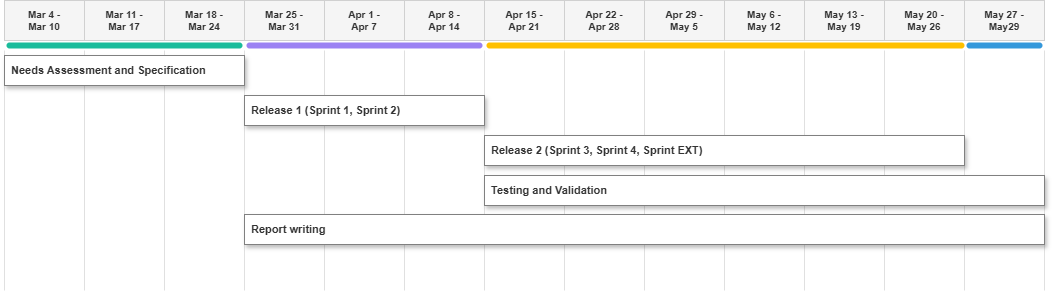
\includegraphics[width=\textwidth]{gantt_diagram.png}
    \caption{Diagramme de Gantt du projet.}
    \label{fig:gantt_diagram}
\end{figure}

\section{Conclusion}
This chapter established the privacy challenges of centralized platforms like Discord, analyzed the SPoF vulnerability of key centralization, and proposed our client-encrypted E2EE + P2P solution. Chapter 2 details the concrete system analysis, requirements specification, and Zero-Knowledge architecture.